\documentclass{article}


\usepackage{amsmath} % math stuff
\usepackage{amssymb} % math stuff
\usepackage{array} % equations and stuff
\usepackage{bm} % bold math
%\usepackage{caption} % suppressed table numbering; incompatible with revtex, and longtable, I think
\usepackage{comment} % comment environment
%\usepackage{enumitem} % customization of enumeration, itemize, and description
\usepackage[T1]{fontenc} % font encoding for special characters, must also use scalable font package
\usepackage[margin=0.8in]{geometry} % paper sizes and margins (but be careful not to mess up pre-defined pages)
\usepackage{graphicx} % for graphics
%\usepackage{helvet} % default font is the helvetica postscript font
\usepackage{lipsum} % lorem ipsum filler text
\usepackage{lmodern} % scalable font?
\usepackage{longtable} % multi-page tables
\usepackage{mathrsfs} % math script font
\usepackage{mhchem} % easier chemical formula
\usepackage{microtype} % allows disabling of ligatures
%\usepackage{newcent} % new century schoolbook font
\usepackage{nicefrac}
\usepackage{parskip} % removes paragraph indentation, and adjusts paragraph skip, as well as list items
%\usepackage{setspace} % adjust text spacing and indents
\usepackage{siunitx} % decimal alignment
\usepackage{subfigure} % divided figures
%\usepackage{tabu} % extra table options
\usepackage{textcomp} % symbols
\usepackage{threeparttablex} % better footnotes with longtable
\usepackage{titling} % title placement
\usepackage{ulem} % strikethrough text
%\usepackage{url} % superceded by hyperref
\usepackage{verbatim} % verbatim environment
\usepackage{xcolor} % colors and color boxes
\usepackage{xspace} % commands that don't eat up white space
\usepackage{hyperref} % links and page setup; should always come last

\hypersetup{
	bookmarks=true,
	colorlinks=true,
	citecolor=blue,
	linkcolor=blue,
	urlcolor=blue,
	pdfstartview={XYZ null null 1.0} % default open view is 100%
}

\DisableLigatures[f]{encoding = *, family = * } % disable ff, fi, fl ligatures, without f option, it also disables -- = endash
\renewcommand{\arraystretch}{1} % extra vertical space in tables

\begin{document}

\pagestyle{empty} % don't number pages

% custom title
\begin{center}
{\LARGE Express Riddler}

\vspace{0.15in}

{\Large 17 July 2020}
\end{center}


\section*{Riddle:}

This year, Major League Baseball announced it will play a shortened 60-game season, as opposed to the typical 162-game season.
Baseball is a sport of numbers and statistics, and so Taylor wondered about the impact of the season's length on some famous baseball records.

Some statistics are more achievable than others in a shortened season.
Suppose your true batting average is .350, meaning you have a 35 percent chance of getting a hit with every at-bat.
If you have four at-bats per game, what are your chances of batting at least .400 over the course of the 60-game season?
And how does this compare to your chances of batting at least .400 over the course of a 162-game season?

\textit{Extra credit}: Some statistics are \textit{less} achievable in a shortened season.
What are your chances of getting a hit in at least 56 consecutive games, tying or breaking Joe DiMaggio's record, in a 60-game season?
And how does this compare to your chances in a 162-game season?
(Again, suppose your true batting average is .350 and you have four at-bats per game.)

\textit{Extra extra credit}: In a 60-game season, what are your chances of \textit{both} batting at least .400 and getting a hit in at least 56 consecutive games?

\section*{Solution:}

Given a probability $p$ of getting a hit (or more generally, a positive outcome) on a single at-bat, the probability $P$ of getting exactly $n$ hits out of $N$ at-bats is given by the binomial distribution:

\[
P=\binom{N}{n}p^{n}(1-p)^{N-n}.
\]

For the current problem, $p=0.35$, $N=4\times60=240$, and the probability must be summed for all $n\geq0.4\times240=96$.
Luckily, all of this can be done in Excel.
I set up the calculation in the file \texttt{Batting\_average.xlsx}.
First I calculated the individual probabilities for each $n$, and summed the answers.
This I called the brute-force calculation.
The result is that for 60 games, the probability is about
\fcolorbox{red}{white}{\bf 6.1\%}\,.
For 162 games, the probability is
\fcolorbox{red}{white}{\bf 0.38\%}\,.

For fun, I also set up a calculator that can take in as input any number of games, number of at-bats per game, true batting average, and desired batting average.
Next I decided to plot how the probability changes as a function of the number of games as well as the true batting averge ($p$).
The plot uses 4 at-bats/game and a desired batting average of 0.4
Here is the result:

\begin{center}
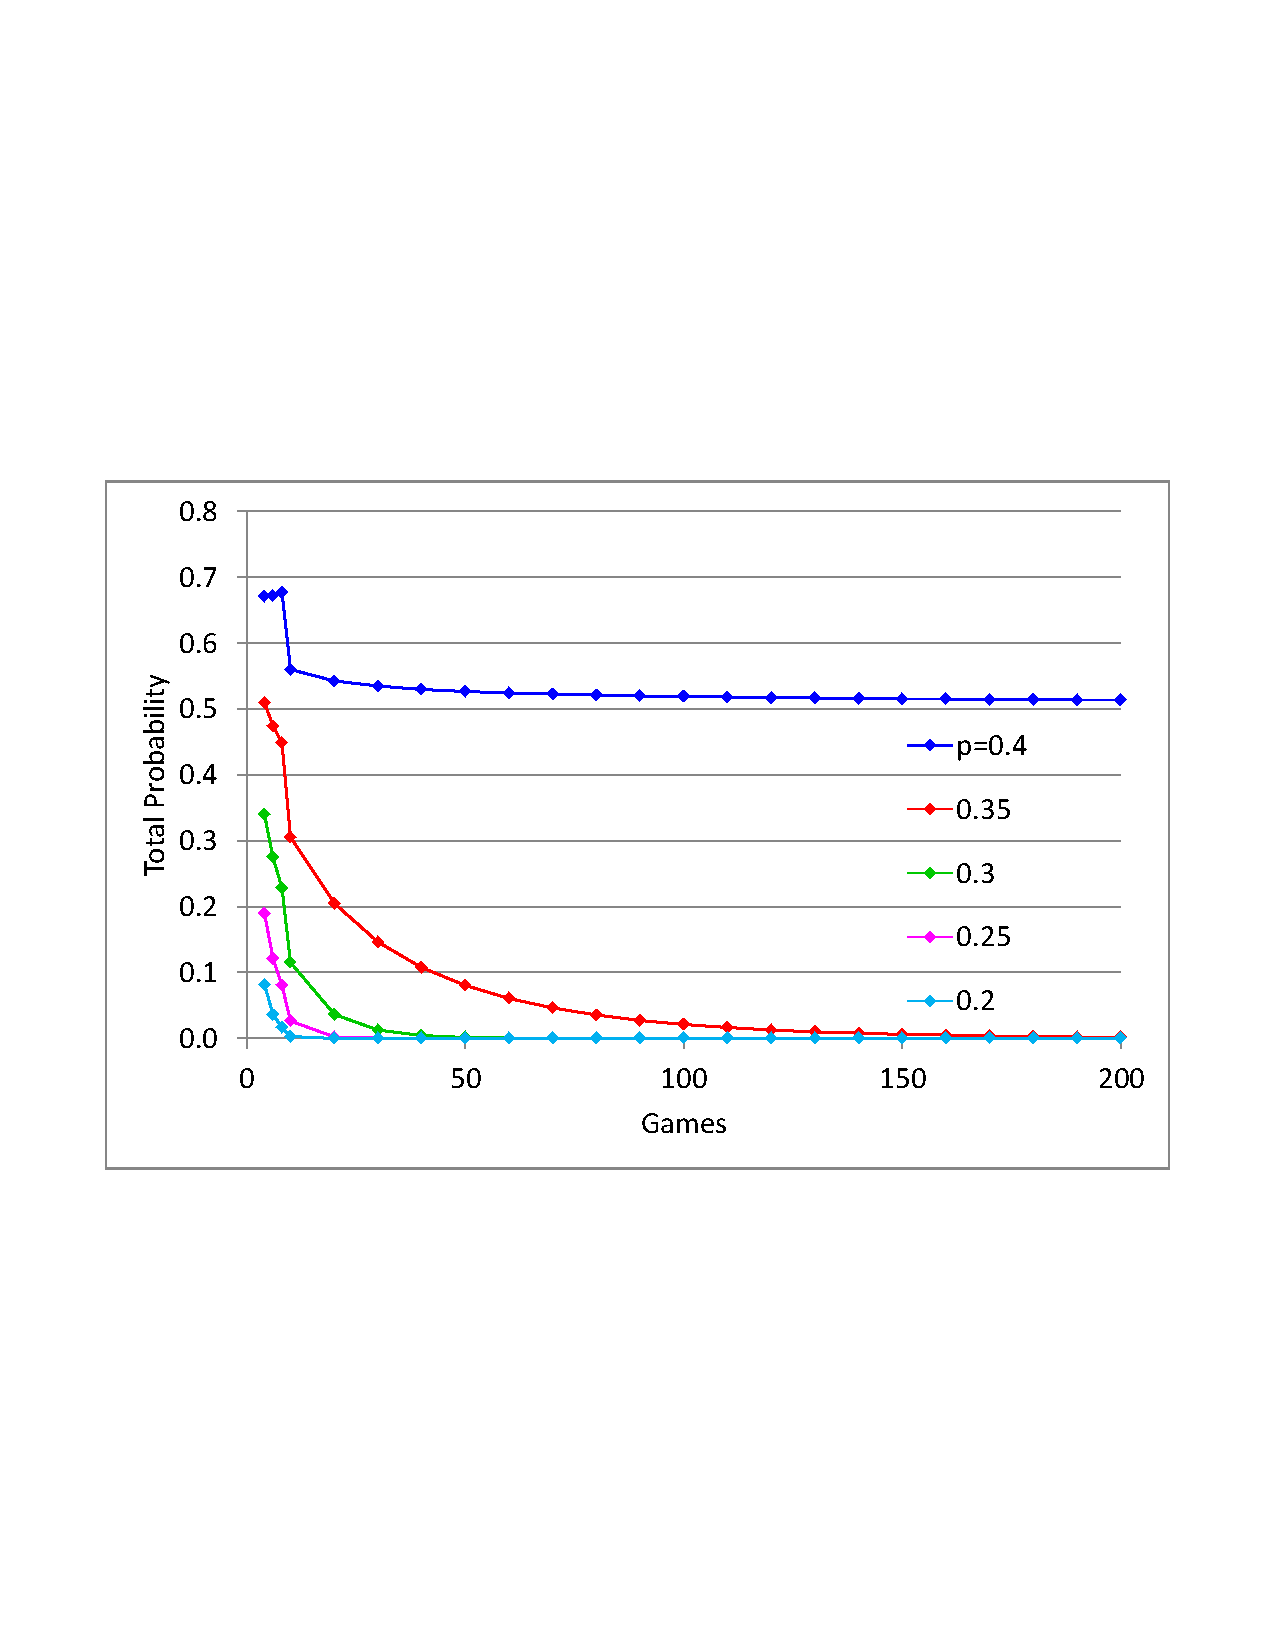
\includegraphics[width=4in, trim=0 3in 0 3in, clip]{Batting_probability.pdf}
\end{center}



\end{document}